\documentclass[11pt]{amsart}

% Standard letter size paper with 1inch margins
\usepackage[letterpaper, margin=1in]{geometry}

% Useful packages 
\usepackage{amsmath, amssymb, amsthm, amsaddr}
\usepackage{enumerate, subcaption, graphicx, hyperref}
\usepackage{algorithm}
\usepackage{algpseudocode}
\usepackage{cite}

\newcommand{\I}{\mathrm{i}}
\DeclareMathOperator{\E}{e}

\title{AMATH 582: Homework 1}
\author{Hunter Lybbert} % first and last name

\address{Applied Mathematics Department, University of Washington, Seattle, WA 
\\ \texttt{hlybbert@uw.edu}}

\date{\today} % you can also just type the date instead of "\today"

\begin{document}

\maketitle

\begin{abstract}
    The following is a detailed explanation and analysis of an application of a method of signal processing to track a signal being emitted from a moving object. We discuss the process of using the Fourier transform and applying a gaussian filter on the transformed signal in the frequency space. We also address the challenges of applying such a method to a high dimensional problem. Various shapes of gaussian filters are considered and analyzed. Potential methods to be applied in the future for further analysis of the object tracking problem are proposed. 
\end{abstract}

\section{Introduction and Overview}\label{sec:Introduction}
Signal processing is a vast field with an array of methodologies as well as applications.
Signal processing is not only relevant to analyzing easily recognizable signals like audio or EKG's but can also be applied to any number of problems where you have some means of gathering data from some signal emitting source.
The problem presented to us in this assignment was to track an unknown submarine moving about in the Puget Sound.
We have been given a broad spectrum recording of acoustics pressure data obtained over 24 hours in half-hour increments.
The data is noisy and requires careful analysis.
In order to track the submarine using the data we aimed to complete the following 3 tasks: \\
\begin{enumerate}
\item Through \textbf{averaging of the Fourier transform} determine the dominant frequency (center frequency)
generated by the submarine. Verify your results through visualization. \\

\item Design and implement a \textbf{Filter} to extract this center frequency in order to denoise the data and
determine a more robust path of the submarine. Visualize the denoised measurement the 3D path of
the submarine and inspect the validity and effectiveness of the denoising. \\

\item Determine and \textbf{plot the} $x$-$y$ coordinates of the submarine path during the 24 hour period. This
information can be used to deploy a sub-tracking aircraft to keep an eye on your submarine in the future.

\end{enumerate}

In the endeavor to track the unknown submarine and complete the requisite tasks we made extensive use of several important Python packages.
Namely, Matplotlib was used to create all plots and animations \cite{Hunter:2007}.
Additionally, NumPy Fast Fourier transform packages including the $n$-dimensional FFT, IFFT, and their respective shift in the Fourier frequency space functions were crucial to the application \cite{harris2020array}.
Moreover there are important theoretical underpinnings behind the algorithm we implemented which will be cited and expounded upon in the following section.

\section{Theoretical Background}\label{sec:theory}
Thus far in class we have discussed methods of signal processing.
The transform which takes center stage in this analysis as eluded to already is the Fourier transform.
For more of a history and details of this transform please see the wikipedia page as a starter reference \cite{wikipedia_fourier_transform}

As introduced in class we have the Fourier Series as follows

\begin{equation}
f(x) = \sum_{k=-\infty}^\infty \hat f_k \E^{\I k x}
\label{eq:fourier_series}
\end{equation}

where each $\hat f_k$ is given by
$$
\hat f_k  = \frac 1 {2 \pi} \int_0^{2 \pi} f(x) \E^{-\I k x} dx.
$$

Additionally we discussed the slightly different variation known as the the Fourier Transform which is given by
\begin{equation}
\hat f_k = \frac 1 {2 \pi} \int_{-\infty}^\infty f(x) \E^{-\I k x} dx
\label{eq:fourier_transform}
\end{equation}

with the inverse Fourier Transform given by

\begin{equation}
f(x) = \int_{-\infty}^\infty \hat f_k \E^{\I k x} dk.
\label{eq:inv_fourier_transform}
\end{equation}

Now in our analysis we are interested in using the Fourier transform to analyze the signal data because it allows us to look at which frequencies are present and what their respective amplitudes or strengths are.
Since our data is so noisy there will be rather many frequencies present but most of them will have a fairly weak amplitude or strength.

This is where we want to utilize some kind of filter to help us weed out these unimportant noisy frequencies.
One such option for filtering (which happens to be the one we want to use) is the gaussian filter.
Applying a gaussian filter allows us to preserve the main frequencies with the strongest amplitudes in the center of the frequency domain, but allows us to mute the many weak frequencies in the long tails outwards.
In our case, the data is three dimensional so we want to use a three dimensional gaussian filter.
If we set the center of the gaussian on the dominant frequency, then the other parameter to change is the value of $\sigma$, the variance, or the shape of the gaussian.
The smaller $\sigma$ is the more rapidly the mass drops off from the gaussian or the larger $\sigma$ is then the slower the drop off is and the more noisy frequencies are retained in the filter.
The value of $\sigma$ is something we can play around with.
Finally the actual equation we will be using for this filter is

\begin{equation}
G = \frac {1}{\sqrt{2 \pi \sigma^2}}\exp \Bigg( - \frac{1}{2 \sigma^2 } \Big( \big(k_x - k_{x_0}\big) + \big(k_y - k_{y_0}\big) + \big(k_z - k_{z_0}\big) \Big) \Bigg).
\label{eq:guassian}
\end{equation}

Let's get into the actual implementation now.

\section{Algorithm Implementation and Development}\label{sec:algorithms}
We will now describe in words and pseudocode the implementation of these methods as we used them in this application to denoise our data and track the submarine.
First, we needed to determine the dominant frequency as described in algorithm \ref{alg:dom_freq}.

\begin{algorithm}
\caption{Determine the Dominant Frequency}\label{alg:dom_freq}
\begin{algorithmic}
\State $ S = {\rm np.load(data)}$ \Comment{Input subdata, after reshaping to (64, 64, 64, 49)}
\State $\hat S$ = fftn(S)
\State $\hat S^\dag$ = fftshift($\hat S$) \Comment{Transformed and shifted subdata (64,64,64,49)}

\State $\hat S^\dag_{\rm avg} = {\rm avg}(\hat S^\dag)$ \Comment{Average computed across time at each point (64,64,64)}
\State $x, y, z = {\rm argmax} \left( {\rm abs} \big( \hat S^\dag_{\rm avg} \big) \right) $ 
\end{algorithmic}
\end{algorithm}

The result of the final step of Algorithm \ref{alg:dom_freq} are the three indices (numbers between 0 and 63) of the location in our cube of average frequency.
What we really want is to know what the frequency value should be to center our gaussian filter from equation \ref{eq:guassian} to use in Algorithm \ref{alg:filter}
We translate these indices into the central frequency of our our gaussian filter by applying these indices to an object representing the frequency space using meshgrid (this is a very python unique implementation detail please refer to code directly).

After indexing this object we will have identified the values which we denote by the coordinate tuple
\begin{equation}(k_{x_0}, k_{y_0}, k_{z_0}) \label{eq:filter_loc} \end{equation}
otherwise known as the center of our gaussian filter.
Now that we have the location of the gaussian filter we can describe the algorithm to actually apply the filter.

\begin{algorithm}
\caption{Apply Gaussian Filter in Frequency Space}\label{alg:filter}
\begin{algorithmic}
\State $ G = \frac {1}{\sqrt{2 \pi \sigma^2}}\exp \Big( - \frac{1}{2 \sigma^2 }\big(k_x - k_{x_0}\big) + \big(k_y - k_{y_0}\big) + \big(k_z - k_{z_0}\big) \Big)$ \Comment{Gaussian Filter using \ref{eq:filter_loc}}
\State $\hat S$ = fftn(S)
\State $\hat S^\dag$ = fftshift($\hat S$)
\State $\hat F^\dag = \hat S^\dag G$ \Comment{Filtered subdata in frequency space still}
\State $\hat F = {\rm ifftshift}(\hat F^\dag)$
\State $F = {\rm ifftn}(\hat F)$ \Comment{Filtered subdata in signal space now}
\end{algorithmic}
\end{algorithm}

Now that we have a filtered signal, $F$, we believe we have eliminated all of the noise so the location of the max signal at any point in time should be the location of our submarine at that time.
Therefore, the final step is to take the argmax($F$) at each time step giving us the indices of the location in the signal space (actual physical space). These results will be described further in following section.

\section{Computational Results}\label{sec:results}
In our work to locate and track the suspected submarine in the puget sound, it was of utmost importance to be able to think through the dimensionality of this problem.
We are tracking a signal from a location in 3 dimensional space, which inherently becomes a 4 dimensional problem.
I had to come up with methods of thinking about what it meant to average something that is 3 dimensional across its fourth dimension (time).
I had to visualize things in lower dimensions in my mind to make sense of the actions that we need to take.
What helped me was to picture a stack of 49 chess boards where each location on a given chess board represented some signal at that time step then the average across time would mean averaging the values in that corresponding location on all 49 chess boards.
Our goal was to do this but as if the chess boards were 3 dimensional themselves.

\begin{figure}[h]
	\centering
	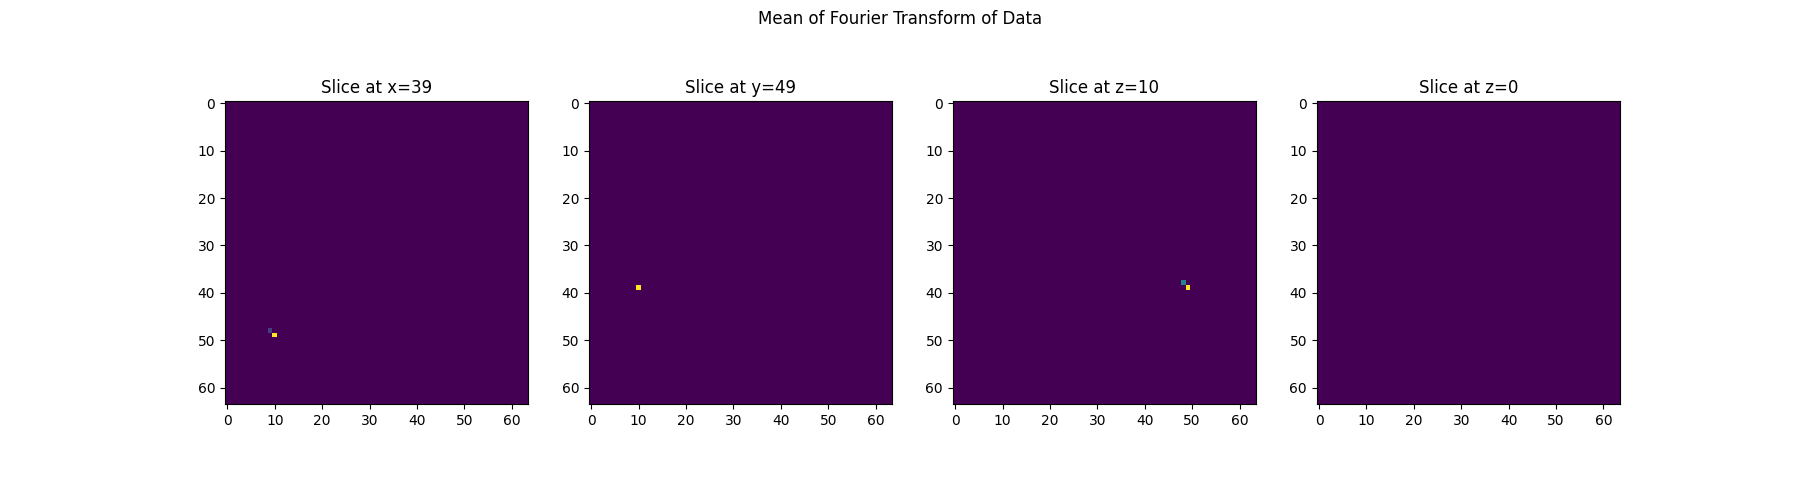
\includegraphics[width=1\textwidth]{../visualizations/visualizing_dominant_frequency.png}
 	\caption{Visualizing each of the 3 slices including the location in our 3 dimensional average frequency object.}\label{fig:f1_0}
\end{figure}

\begin{figure}[h]
	\centering
	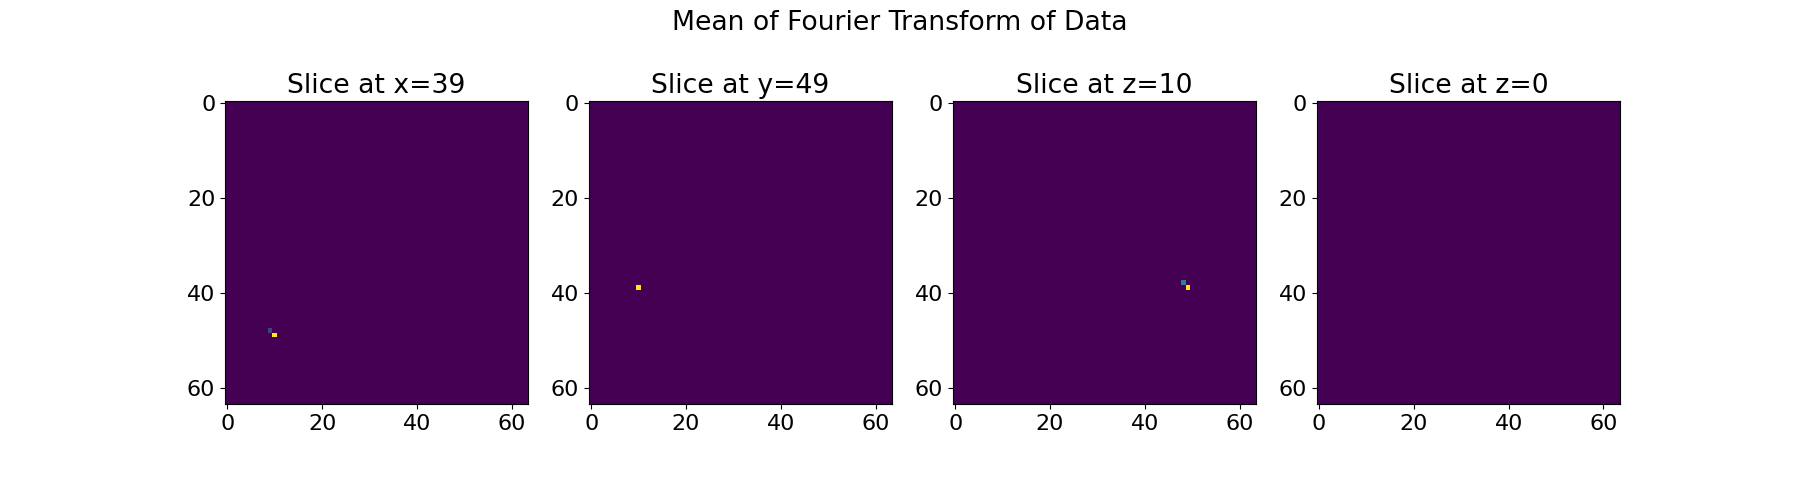
\includegraphics[width=1\textwidth]{../visualizations/visualizing_dominant_frequency_plus.png}
 	\caption{Visualizing each of the 3 slices including the location in our 3 dimensional average frequency object. We also visualize a slice which does not intersect the max frequency in order to convey how drastic the location of the max frequency is. In order to show this comparison things have been rescaled here.}\label{fig:f1}
\end{figure}

One way to visualize the result of finding the max average frequency was to take slices of the average frequencies across time to confirm what we found by calculation.
As seen in Figures \ref{fig:f1_0} and \ref{fig:f1} by looking at the slices corresponding to the location of the max frequency in our cube of frequencies, we see the bright location corresponding to the location we found to be the max frequency.

This helped confirm that I had identified the correct dominant frequency at which to center the gaussian filter to help us eliminate the noise.
Furthermore we visualized the path of the of the submarine in Figure \ref{fig:f2}

\begin{figure}[h]
	\centering
	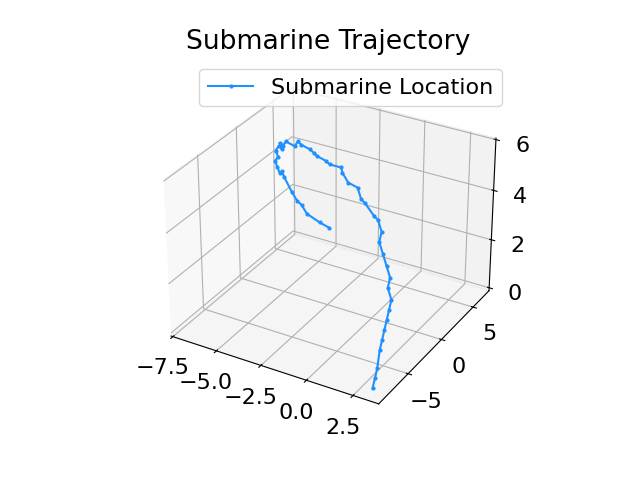
\includegraphics[height=2in]{../visualizations/submarine_static_3d.png}
 	\caption{The resulting path in 3 dimensions that we determined after applying Algorithms \ref{alg:dom_freq} and \ref{alg:filter}. In this iteration of the filter we used $\sigma=1.3$.}\label{fig:f2}
\end{figure}

\begin{figure}[h]
	\centering
	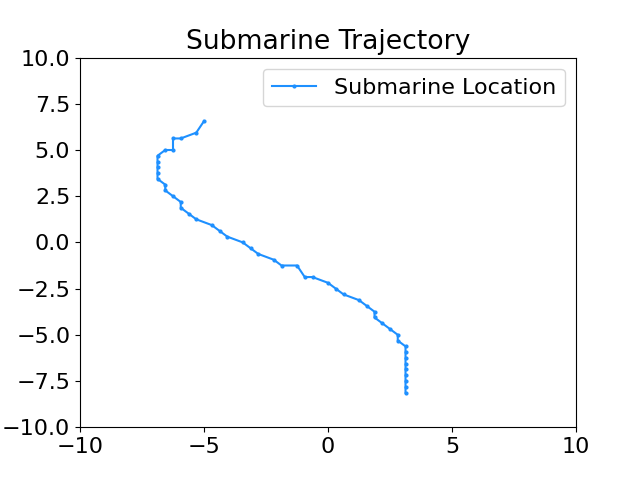
\includegraphics[height=2in]{../visualizations/submarine_static_2d.png}
 	\caption{This is just the 2 dimensional projection of the path given in the above 3d plot. The same value of $\sigma$ was used in the filter.}\label{fig:f3}
\end{figure}

Moreover, I was able to generate several other important visualizations in gif form which are viewable on my Github.
Click \href{https://github.com/hunter-lybbert/uw-central/blob/data-analysis-hw-1/data_analysis/hw_01/visualizations/submarine_trajectory_3d.gif}{here} for the animation of the 3 dimensional path and click \href{https://github.com/hunter-lybbert/uw-central/blob/data-analysis-hw-1/data_analysis/hw_01/visualizations/submarine_trajectory_2d.gif}{here} for the animation of the path in just the $x$-$y$ plane ($z = 0$).

\section{Summary and Conclusions}\label{sec:conclusions}
We are pleased with the results we have thus far and are aware of several ways to improve our work in the future.
I would first revisit this and create plots for various values of $\sigma$ the parameter in the gaussian filter.
I manually performed this analysis but ran out of time to include it in this article.
Secondly, I would like to continue observing the ``Submarine" and gather more data.
More data would enable us to inform what the hyperparameters of our gaussian filter such as the location (mean) and the shape (variance) aught to be such.
Additionally we chose a uniform variance for each dimension, perhaps we would get some interesting results if we had a difference variance for each dimension in the gaussian filter.
More data would also enable us to validate our tracking method.
We currently lack a ground truth of sorts to help us know if we have actually identified the right path of the submarine.
This is one of the main drawbacks of our results so far.

\section*{Acknowledgements} 

The author is thankful to Jaxon Tuggle for useful discussions about the process to find the dominant frequency in task 1. 
Additionally Hailey Sparks was thoroughly helpful when comparing methods by which we identified the correct location of our gaussian filter for task 2.
We would also like to thank Professor Eli Shlizerman for carefully instructing us in class and answering questions in Office Hours.
Finally, it is necessary to thank the following students Nate Ward, Sophie Kamien, and Mikelle Rogers, whose questions helped clarify understanding of the algorithm we implemented by giving chances to explain ideas and debug code together.

\bibliographystyle{abbrv}
\bibliography{references_hw1} % make sure this matches the .bib file for your corresponding document. You also have to maintain your references in the .bib file 

\end{document}
